\documentclass{article}

\usepackage[utf8]{inputenc}
\usepackage{fancyhdr}
\usepackage[french]{babel}
\usepackage{graphicx}

\pagestyle{fancy}

\renewcommand{\contentsname}{Table des matières}

\fancyhead[L]{Knights of the \\Fallen Lemon}
\fancyhead[C]{\textbf{Company \& Co.}}
\fancyhead[R]{Janvier 2018}

\begin{document}
\begin{titlepage} 
	\begin{center}
	\line(1,0){300}\\
	[2mm]
	\huge{\bfseries Company \& Co. \\Cahier des charges}\\
	[1mm]
	\line(1,0){200}\\
	[1.5 cm]
	\textsc{\LARGE Knights of the Fallen Lemon}\\
	[0.75 cm]
	\textsc{\Large Victor HACQUARD\\Maya HANNACHI\\Malo LECOMTE\\Léa MASSELLES}\\
	[1 cm]
	\textsc{\large 19 Janvier 2018}
	\end{center}
\end{titlepage}

\tableofcontents
\newpage

\addcontentsline{toc}{section}{Introduction}
\section*{Introduction}
Créer un jeu de toutes pièces n'est pas une mince affaire. En créer un qui sera à la fois loufoque et appréciable, encore moins.
De l'ambition, nous en avons. Du sérieux également, tout autant que notre humour omniprésent et décalé.

Cet ouvrage a été écrit dans le but de vous présenter et de vous expliquer nos idées pour notre projet de première année, ainsi que l'avancement probable de nos travaux et de nos efforts.

Notre groupe, Knights of the Fallen Lemon, vous présentera ici son projet de jeu, Company \& Co., qui sera le fruit de notre sueur et de nos larmes, fussent-elles de désespoir... ou de rire.
\section{Membres de l'ordre des chevaliers}
\vspace{0.3cm}\hspace{-0.7cm}
\textbf{Victor "Zexeed" HACQUARD}
\begin{itemize}
\item[•] \textbf{\textit{Classe}} : Entité supérieure
\item[•] \textbf{\textit{Age}} : 19 ans
\item[•] \textbf{\textit{Caractéristiques}} : Plus de café que de sang dans l'organisme
\item[•] \textbf{\textit{Capacité spéciale}} : Beaucoup de résultats, peu de travail
\item[•] \textbf{\textit{Devise}} : "Never say no to panda."
\end{itemize}

En tant que grand fan de jeux vidéos, je me suis déjà essayé plusieurs fois à la programmation de petits jeux (en C++), sans que ces derniers ne soient très perfectionnés. Ce projet est donc l'opportunité parfaite de m'améliorer et d'aquérir de nouvelles connaissances.

J'ai développé l'essentiel de mes connaissances en programmation lors d'un projet  de traitement d'image en C effectué l'année dernière à l'EPFL. Ce projet, bien que de moins grande envergure, m'a habitué aux longues nuits passées à programmer quelques jours avant le rendu et m'a permis d'apprendre certaines logiques et mécaniques qui pourront être utiles cette année.\\
\\
\vspace{0.3cm}
\textbf{Maya "Katynkae" HANNACHI}
\begin{itemize}
\item[•] \textbf{\textit{Classe}} : Distributeur de câlins
\item[•] \textbf{\textit{Age}} : 18 ans
\item[•] \textbf{\textit{Caractéristiques}} : Adepte du diabète liquide 
\item[•] \textbf{\textit{Capacité spéciale}} : Appel à un ami : Voltaire
\item[•] \textbf{\textit{Devise}} : Le dinar algérien. "Comment ça je n'ai pas compris ?"
\end{itemize}

Si, comme la majorité des étudiants de cette école, j'apprécie un bon jeu vidéo, je n'ai jamais réalisé de projet de cette envergure, ou de projet informatique tout court, pour être honnête. 
En réalité, j'ai découvert la programmation en arrivant à EPITA en septembre dernier. Mes compétences et mes connaissances en la matière sont donc encore au stade embryonnaire.
Ce sont justement mes attentes vis-à-vis de ce projet : apprendre, découvrir, un premier pas vers la maîtrise. Le C\# est une nouveauté, Unity aussi, et j'ai bien l'intention d'y remédier.
(Le LaTeX, par contre, je connais ! C'est toujours ça de pris.)\\
\\
\vspace{0.3cm}
\textbf{Malo "BKN" LECOMTE}
\begin{itemize}
\item[•] \textbf{\textit{Classe}} : Mage demi-dragon
\item[•] \textbf{\textit{Age}} : 17 ans
\item[•] \textbf{\textit{Caractéristiques}} : Homme appareillé incurvé
\item[•] \textbf{\textit{Capacité spéciale}} : Effectue le dab dans des endroits inadéquats
\item[•] \textbf{\textit{Devise}} : "Les loutres, Lutrinae, sont une sous-famille de mammifères carnivores de la famille des Mustélidés."
\end{itemize}

Fan de jeux vidéos depuis mon plus jeune âge (vive Nintendo), je ne me suis penché sur la programmation que récemment grâce à la spécialité ISN en terminale. Cela m'a poussé à rejoindre l'EPITA car j'ai trouvé une passion pour l'informatique (au-delà du gaming).

J'ai par ailleurs eu l'occasion de réaliser un petit projet sur quelques mois, un jeu de plateformes. Certes, ce projet était moins imposant que ce que l'on nous demande pour ce 
second semestre mais il m'a permis d'acquérir quelques compétences pour la gestion d'un projet. De plus, les TP effectués depuis le début de l'année m'ont également permis d'obtenir
de bonnes bases en C\#. Il ne me reste plus qu'à apprendre UNITY et me perfectionner en C\# afin de maîtriser les nombreuses applications que ce langage rend possibles.\\
\\
\vspace{0.3cm}
\textbf{Léa "Lemasyma" MASSELLES (Chef de projet)}
\begin{itemize}
\item[•] \textbf{\textit{Classe}} : Petite mère
\item[•] \textbf{\textit{Age}} : 18 ans
\item[•] \textbf{\textit{Caractéristiques}} : Beaucoup de colère dans un petit corps
\item[•] \textbf{\textit{Capacité spéciale}} : Anti-procrastination
\item[•] \textbf{\textit{Devise}} : "See you space cowboy"
\end{itemize}


Les jeux vidéos m'attirent depuis toute petite, mais c'est également une passion qui m'a poussé à m'intéresser de plus près à l'informatique de manière générale. J'ai déjà dû coder quelques petits programmes, comme un serveur local pour jouer avec des amis au même jeu, ou de plus grands projets, comme un court jeu vidéo pour mon projet de fin d'année en ISN. A chaque fois, être sur un ordinateur à écrire dans un langage que personne ne comprend, à moins d'y être initié, et voir le résultat de mes efforts après des heures de travail, ça me plaisait.


C'est pour cela que je suis à l'EPITA et que je travaille sur ce projet, je veux continuer à approfondir cette passion pour l'informatique. Je n'ai jamais codé en C\# et UNITY auparavant, et pouvoir maîtriser un nouveau langage de programmation ne fait jamais de mal, surtout si vous vous destinez à être ingénieur informaticien.

\section{Le projet de manière générale}
\subsection{Origine du projet}
Trouver une idée de projet peut être légèrement compliqué. Chaque membre avait plusieurs propositions, mais nous en avons retenu deux que nous avons fusionné. L'une a été trouvée par Victor au début du projet, consistant à créer un jeu se déroulant dans une entreprise avec des personnages très caricaturaux. L'autre provient de Malo, très inspiré par son amour pour les jeux vidéos, imaginant un gameplay se basant sur la gestion d'unités individuelles qui, réunies ensembles et si bien maitrisées, deviennent plus puissantes et permettent de vaincre l'ennemi, concept que nous verrons plus en détails dans la section suivante.

\subsection{Le scénario}
Nous avons imaginé que le jeu se déroulerait dans une entreprise, où nous incarnons un stagiaire en bas de l'échelle hiérarchique, désespéré par sa situation. Il déciderait de quitter son poste pour fonder sa propre affaire et prendre sa vie en main. Il devra alors combattre les entreprises concurrentes tout en gérant la sienne et ses employés pour gagner des parts de marché et devenir le meilleur, et éventuellement devoir affronter ses anciens collègues et supérieurs pour prendre sa revanche.

\subsection{Le but du jeu}
Notre jeu n'est pas à prendre au premier degré. Le but est vraiment de faire un jeu humoristique parsemé de blagues qui ne feraient rire que des personnes de notre génération. Toutefois, ce n'est pas parce qu'il présentera un aspect drôle qu'il ne donnera pas du fil à retordre aux joueurs. La difficulté augmentera bien au fur et à mesure, et nous espérons que notre humour détendra le joueur pour ne pas le voir abandonner au milieu d'une partie.

\subsection{Une expérience utile}
Nous espérons que ce projet peut nous offrir un exemple concret du déroulement du travail en groupe, et peut-être nous donner une idée de la vie en entreprise. En sept mois, nous avons le temps de mettre en place une méthodologie pour travailler efficacement en groupe, méthodologie que nous pourrons probablement utiliser dans un futur proche.

De manière individuelle, nous pourrons améliorer nos capacités pour travailler et apprendre en autonomie. Si nous répartissons le travail de manière correcte, chacun pourra maitriser le langage C\# et Unity et réutiliser ses connaissances dans de futurs projets, voire dans notre vie active.

\section{L'aspect technique}
\subsection{Le gamedesign}

\subsubsection{Le gameplay : à mi-chemin entre tactical RPG et le jeu de gestion}

Comme évoqué précédemment, le gameplay de notre jeu se basera sur la gestion d'unités individuelles qui devront être combinées pour pouvoir vaincre les ennemis. En termes légèrement plus techniques, le jeu sera un \textit{tactical RPG}, abrégé \textit{T-RPG}, où le joueur devra gérer plusieurs types de personnages.\\

Les T-RPG sont des jeux de rôle tactiques. Le joueur doit gérer chaque personnage un à un et prendre en compte ses forces et ses faiblesses, trouver des stratégies ingénieuses, comme exploiter les failles de ses ennemis, pour pouvoir combattre l'adversaire efficacement.\\

Une des caractéristiques principales des T-RPG est que le joueur doit gérer un nombre d'unités important. Dans les jeux de rôle plus "classiques", le joueur doit souvent incarner une seule personne ou gérer une équipe comptant six membres au maximum, alors que ce nombre peut s'avérer beaucoup plus élevé dans le cas d'un T-RPG. De même pour le camp adverse, comptant un nombre d'unités ennemies équivalent à celui du joueur.\\

\textit{Company \& Co.} sera également un jeu de tour par tour, le joueur devra donner une action à chacune de ses unités pendant un tour.\\

D'un autre côté, le jeu sera également axé sur la gestion. Hors des combats, vous allez devoir gérer votre équipe et gérer votre entreprise, et ce de façon très simple.\\

Vous pourrez augmenter le niveau de vos unités, de vos armes, et même recruter de nouveaux employés. Vous pourrez voir votre entreprise se développer de plus en plus
jusqu'à atteindre le niveau maximum.

\subsubsection{Les personnages}
Chaque personnage de T-RPG doit avoir des capacités spéciales exploitables, pouvant mener à différentes stratégies. Nous évoquerons plusieurs caractéristiques au sein de chaque classe, comme les points d'attaque, de défense ou de vie, composants les statistiques des personnages, en plus des capacités spéciales. Il sera possible d'évoluer au sein de ces classes et dans certains cas de changer de classe. Nous avons donc imaginé plusieurs types d'unités.

En plus de ces capacités, les personnages auront aussi leur utilité propre dans la partie "Tycoon" du jeu, il sera donc nécessaire de bien gérer les employés pour le bien de l'entreprise.\\

\begin{itemize}
\item[•] \textbf{\textit{Stagiaire}} : L'unité la plus faible en termes de statistiques, mais c'est aussi la moins cher a employer. Il peut remonter les points de vie des personnages alliés et les empêcher de dormir pendant un certain temps en leur apportant du café. (pendant entre 2 et 5 tours)\\
\item[•] \textbf{\textit{Secrétaire}} : Caractéristiques légèrement inférieures à celles des stagiaires à l'exception de la vitesse qui est supérieure. En plus de rendre des points de vie, son café augmente temporairement les statistiques du personnage.\\
\item[•] \textbf{\textit{Technicien de surface}} : Possède une attaque élevée, au détriment de sa défense. Sa caractéristique particulière est de voir les dégats infligés augmentés lorsque l'ennemi se trouve sur une case qui a été nettoyée.\\
\item[•] \textbf{\textit{Agent de sécurité}} : L'inverse du technicien de surface, une défense élevée et une grande quantité de points de vie. Force les ennemis autour de lui à l'attaquer (capacité de taunt)\\

\item[•] \textbf{\textit{Ingénieur}} : Unité attaquant à distance et possédant une attaque mentale élevée. Hors combat, il peut créer des armes ou les améliorer.\\
\item[•] \textbf{\textit{Comptable}} : Unité attaquant aussi à distance mais spécialisée dans la défense et la défense mentale. Sa force principale est sa capacité passive à endormir les personnages présents dans un certain rayon autour de lui. Il peut aussi diminuer les statistiques des ennemis grâce à ses talents d'optimisation fiscale.\\
\item[•] \textbf{\textit{Manager}} : Cette classe compte très peu de points de défense mais beaucoup de points d'attaque. Après un combat contre un manager, si ce dernier gagne, il prend alors le contrôle de l'unité adverse.\\
\item[•] \textbf{\textit{PDG}} : Une unité ayant très peu de points d'attaque et peu de points de vie mais à la capacité spéciale surpuissante. Il peut invoquer jusqu'à 4 intérimaires, ensuite contrôlables à volonté. Cependant, ces derniers disparaissent à la fin du combat et ne font pas partie de l'entreprise.\\
\end{itemize}

Une autre classe additionnelle est celle d'espion industriel. C'est une classe qui s'ajoute à la classe d'un personnage existant via une formation. Un espion industriel ne fait plus partie de l'entreprise dans la partie "Tycoon" du jeu mais a une chance d'être présent dans l'équièe adverse lors des combats. Le joueur peut alors récupérer le contrôle de cette unité dès qu'il le souhaite. Cependant, lorsque l'espion change de camp, il devient alors la cible prioritaire de l'ennemi.

\subsubsection{Les objets}

Il y aura différents types d'objets, utilisables par les personnages en fonction de leur classe et de leur niveau. Ils seront divisés en deux catégories distinctes : les objets spécifiques à une classe et ceux utilisables par tous.\\
Les objets de base pourraient être améliorés jusqu'à deux fois, à mesure que l'entreprise se développe et que le joueur progresse dans l'aventure.
Parmi les objets spécifiques, on trouve notamment : \\
\begin{itemize}
\item[•] \textbf{\textit{La thermos de café}} : spécifique aux classes stagiaire et secrétaire, elle permet de transporter une certaine quantité de café, augmentant au fur et à mesure des améliorations. Tout le monde apprécie une bonne tasse de ce doux breuvage, n'est-ce pas ? Ils seront toujours disponible pour en apporter.\\
\item[•] \textbf{\textit{Le taser}} : spécifique à l'agent de sécurité, il permet d'immobiliser un ennemi pendant un tour. Il nécessite cependant entre 3 et 5 tours pour se recharger avant de pouvoir être utilisé à nouveau. Ce temps diminue lui aussi avec les diverses améliorations.\\
\item[•] \textbf{\textit{Les doughnuts}} : augmente les statistiques de celui qui le mange mais inflige une pénalité de points de vie. Seul l'agent de sécurité ne subit pas cet effet négatif car ses longues années d'expérience de dégustation de ces mets délicats l'y ont habitué.\\
\item[•] \textbf{\textit{Les diverses armes}} : De la calculatrice à l'ordinateur pour l'ingénieur et le comptable, les trombones ou l'agrafeuse pour les stagiaires et secrétaires, la matraque pour l'agent de sécurité et des liasses de billets verts pour le PDG et le manager.
\end{itemize}

\subsubsection{Les statistiques}
Qu'est-ce qui montre qu'un personnage est "fort" ou "faible" ? Ses statistiques. Intrinsèquement liés au personnages, elles sont à la base de ses capacités et de son comportement au combat.\\

\begin{itemize}
\item[•] \textbf{\textit{Attaque}} : puissance des attaques physiques portées aux adversaires\\
\item[•] \textbf{\textit{Défense}} : résistances aux attaques physiques\\
\item[•] \textbf{\textit{Attaque Mentale}} : puissance des attaques mentales (ou à distance) portées aux adversaires\\
\item[•] \textbf{\textit{Défense Mentale}} : résistances aux attaques mentales\\
\item[•] \textbf{\textit{Vitesse}} : nombre de cases où le déplacement de l'unité est possible\\
\item[•] \textbf{\textit{Agilité}} : nombre d'attaques portées en un tour\\
\item[•] \textbf{\textit{Charisme}} : influe sur les améliorations apportées par les personnages de soutien (un charisme élevé permet de meilleurs boosts de statistiques)\\
\end{itemize}

Ainsi, le nombre de dégâts subis lors d'une attaque physique de l'adversaire seraient proportionnels à l'attaque de l'ennemi et à la défense de l'unité jouée. Le principe est le même pour les attaques mentales.\\

Une autre statistique, la \textbf{\textit{Notoriété}}, ne serait pas liée aux personnages mais à l'entreprise dans son ensemble. Elle dépendrait directement des résultats des combats : l'état final des unités, la quantité d'unités K.O. au cours du combat...  En somme, comment vous vous comportez avec vos employés ! Et mieux vous les traitez, plus vous serez récompensés. Comment ? En obtenant la possibilité de se procurer des unités plus puissantes et moins chères. La qualité à bas prix.

\subsection{Le langage de programmation}
Vous vous en doutez, pour créer un jeu vidéo, nous avons besoin de quoi coder. Comme proposé dans la partie \textbf{Restrictions} du \textbf{Dossier Projet Informatique}, nous utiliserons C\# accompagné de UNITY. 

Utiliser ces deux derniers nous procurent beaucoup d'avantages. Concernant C\#, il s'agit du langage que nous maîtrisons tous le plus grâce aux multiples TP dessus. De plus, nous avons éliminé Caml d'office avant le début du projet, le trouvant trop compliqué à utiliser pour coder, même des fonctions simples.

Quant à UNITY, nous suivons la lignée de la majorité des projets précédents de Sup. Nous pensons, et non pas parce que c'est une restriction, qu'il pourrait être très utile dans la création de notre jeu d'un point de vue mécanique et graphique, grâce aux assets disponibles en ligne.

\subsection{Les graphismes}
Comme pour la majorité des T-RPG et jeux de gestion, notre jeu sera affiché en 2.5D. Vous l'aurez probablement deviné, la 2.5D est un mi-chemin entre la 2D et la 3D. Le terme ne désigne pas de méthode spécifique, mais plutôt tout un ensemble. 

Pour la partie combat, nous pensions afficher des sprites, c'est-à-dire des images représentant les personnages, en 2D sur un décor en 3D où ils pourront se déplacer dans plusieurs directions. De même pour la partie gestion, les seuls changements étant ceux du gameplay.


\subsection{L'Intelligence Artificielle}
Pour la partie sur l'intelligence artificielle, plusieurs problématiques vont venir. Nous allons commencer par créer une intelligence artificielle "bête" mais fonctionnelle.

Dans ses débuts, cette intelligence artificielle va donc avoir pour but de se déplacer vers l'ennemi le plus proche et de l'attaquer. Nous pourrons pour cela utiliser l'algorithme du pathfinding A* qui permet de trouver le chemin le plus court d'un point A à un point B en un temps minimal.

Au cours de ses améliorations, l'intelligence artificielle va pouvoir ensuite sélectionner quelle est la meilleure stratégie entre les distances et les forces et faiblesses. Elle pourra également déterminer s'il vaut mieux attaquer ou battre en retraite ou alors utiliser des objets.
Il faudra donc créer un algorithme rapide pour prendre tout cela en considération, sans perdre du temps à chaque tour de l'IA.


\subsection{Multijoueur}
Le multijoueur se baserait sur un système de classement entre entreprises se basant sur son capital, c'est-à-dire sur l'argent qu'elle possède. Un joueur pourra envoyer une demande de défi à un autre, ce dernier pouvant l'accepter ou la refuser. S'il accepte, les deux joueurs pourront s'affronter en face à face.	Le gagnant recevra une partie de l'argent du perdant et gagnera des places dans le classement.

\section{Nos inspirations}
\subsection{Histoire}
La partie histoire est très inspirée des mécanismes de jeux de gestion, en particulier par tous les jeux de types \textit{Tycoon}, comme \textit{Game Dev Tycoon}, la série des \textit{RollerCoaster Tycoon}, ou même \textit{Jurassic Park: Operation Genesis}. Tous ces jeux ont un même principe : créer une entreprise, la développer et la gérer pour qu'elle reste viable.

\subsection{Gameplay}
La plus grande inspiration pour le gameplay est la série des jeux \textit{Fire Emblem}. Tous sont très connus et la façon dont chaque personnage est mis en place, combiné avec les mécaniques de gameplay, comme les relations entre personnages augmentant leurs statistiques au combat, nous ont donné beaucoup d'idées.

\subsection{Graphisme}
Les jeux de gestion ainsi que les T-RPG, comme dit précédemment, sont en majorité en 2.5D. Les jeux évoqués ci-dessus ont des graphismes en 2.5D :


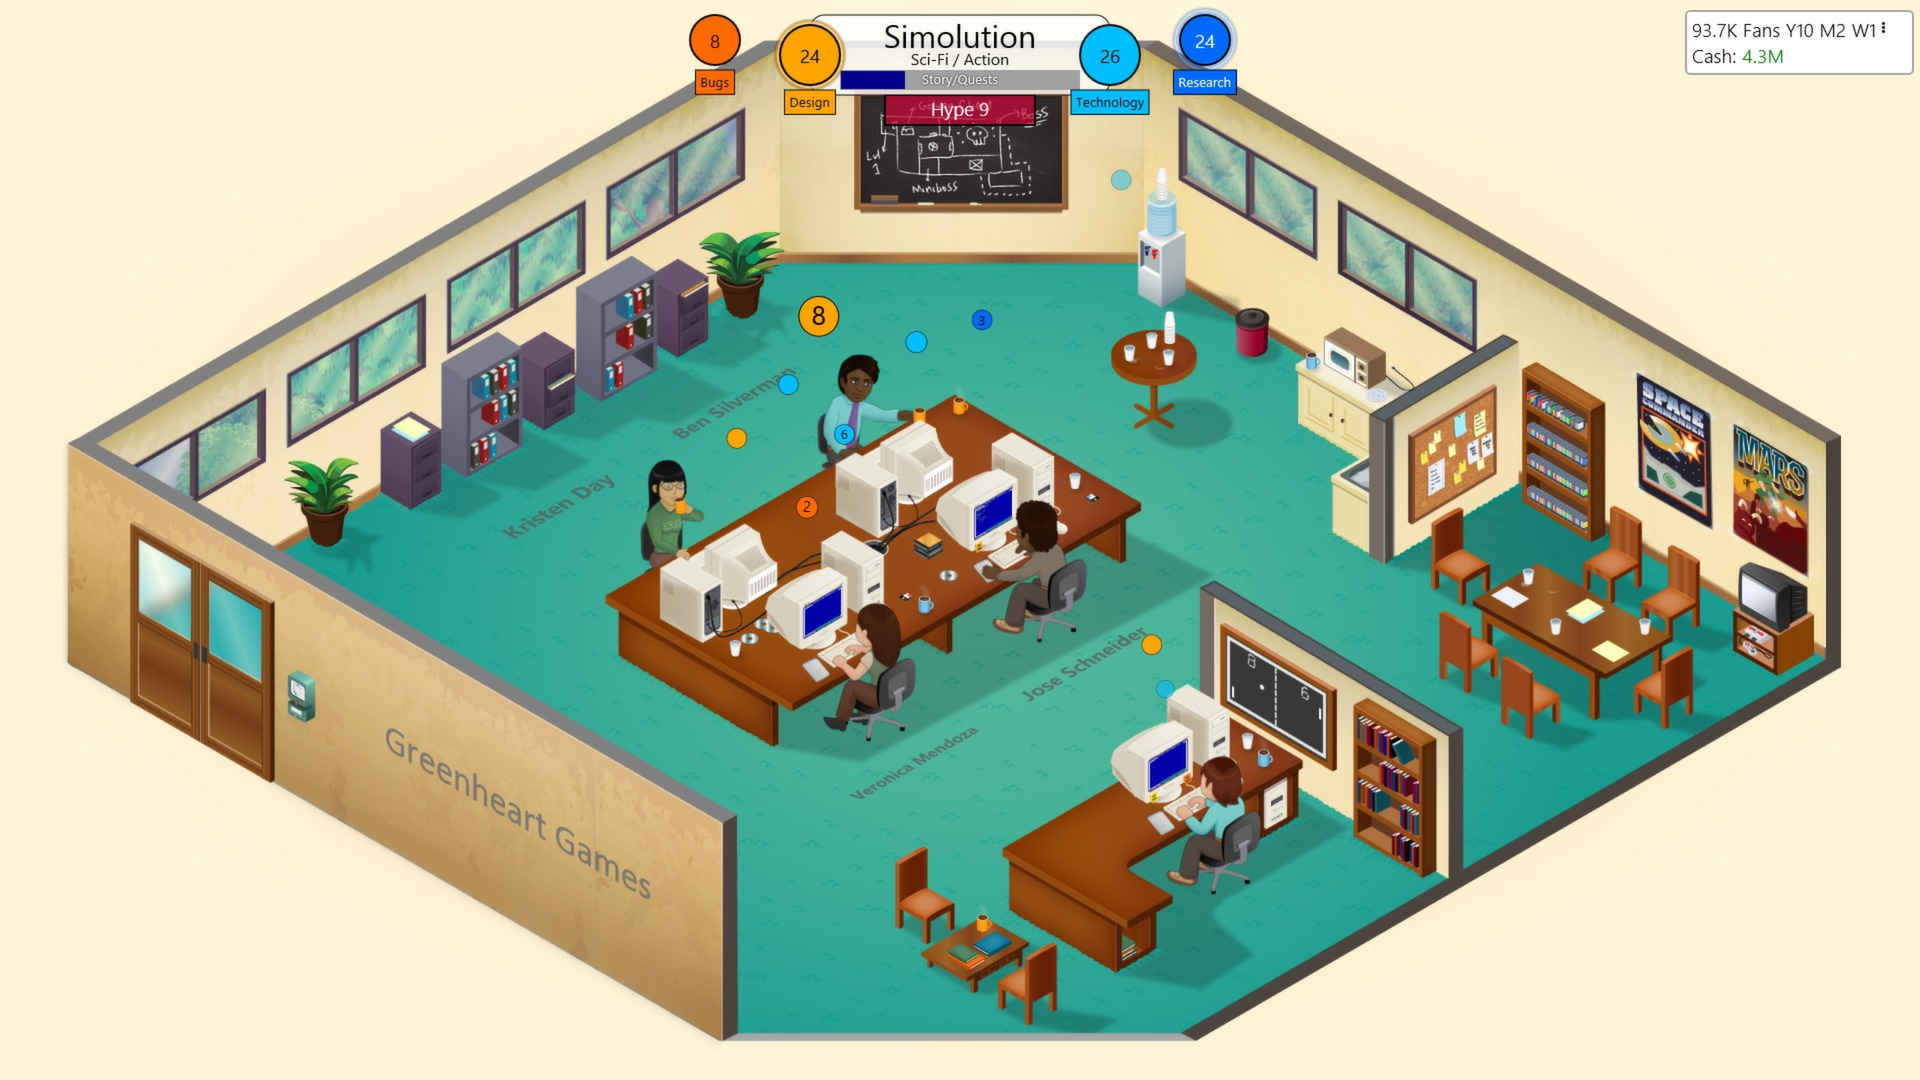
\includegraphics[width = 5.5cm]{gamedev.jpg} \hspace{10 pt} 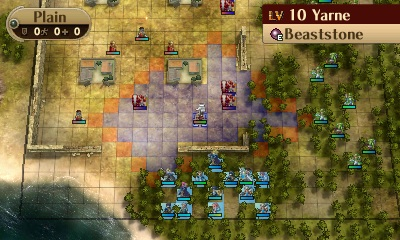
\includegraphics[width = 5.1805cm]{18-10.jpg}\\  \scriptsize \hspace{50 pt}Image tirée de Game Dev Tycoon \hspace{75 pt} \scriptsize Image tirée de Fire Emblem Awakening



\section{Planning et développement}
\subsection{Répartition des tâches}
\begin{center}
	\begin{tabular}{|c||c|c|c|c|}
	\hline
    \textbf{Tâches} & \textbf{Victor} & \textbf{Maya} & \textbf{Malo} & \textbf{Léa} \\ \hline
    Graphismes & $-$& & & $+$\\ \hline
    Musiques et son & $+$& $-$& & \\ \hline
    Game design & $+$ & $-$ &  & \\ \hline
    Créations des menus & & $+$& $-$& \\ \hline
    Gameplay & & & $+$ & $-$\\ \hline
    IA & $-$ & & $+$&\\ \hline
    Multijoueur & &  & $-$&$+$\\ 
    \hline
    Développement Web &  & $+$ & & $-$\\ \hline
	\end{tabular}
\end{center}
Légende:\\
\hspace*{1cm}-Responsable: $+$ \\
\hspace*{1cm}-Suppléant: $-$

Chacun d'entre nous s'est vu assigner deux tâches principales en tant que responsable et deux en qualité de suppléant. 

\subsection{Avancement du projet}
\begin{center}
   \begin{tabular}{ | c || c | c | c | }
     \hline
 	 \textbf{Soutenance} & \textbf{1} & \textbf{2} & \textbf{3}    \\ \hline
     Graphismes & 10\% & 40\% & 100\% \\ \hline
     Musiques et Son & 0\% & 20\% & 100\% \\ \hline
     Game design & 50\% & 80\% & 100\% \\ \hline
     Création des menus & 5\% & 60\%  & 100\% \\ \hline
     Gameplay & 50\% & 80\%  & 100\% \\ \hline
     IA & 0\% & 20\%  & 100\% \\ \hline
     Multijoueur & 50\% & 80\% & 100\% \\ \hline
     Développement Web & 40\% & 75\% & 100\% \\ \hline
   \end{tabular}
 \end{center}

Il est à noter que les pourcentages sont donnés à titre indicatif, avec une marge d'erreur de 10\% au maximum. Les pourcentages représentent des portions du travail final.

\addcontentsline{toc}{section}{Conclusion}
\section*{Conclusion}
Pourquoi hésiter entre plusieurs types de jeux quand on peut les combiner ? Tycoon et T-RPG, combat et gestion, bourrin et réflexion : tel est notre projet. Knights of the Fallen Lemon sont là pour vous présenter \textbf{Company \& Co.}, qui pourrait bien devenir polyvalent, et surtout... amusant, tant à créer qu'à jouer. 



\end{document}
